
\documentclass{beamer}
\usepackage{amsmath}
\usepackage{amssymb}
\usepackage{dsfont}
\usepackage{unicode-math}
\usepackage{verbatim}
\usepackage{xeCJK}
\mode<presentation> {
\setbeamertemplate{footline}[frame number]
\beamertemplatenavigationsymbolsempty
% The Beamer class comes with a number of default slide themes
% which change the colors and layouts of slides. Below this is a list
% of all the themes, uncomment each in turn to see what they look like.

%\usetheme{default}
%\usetheme{AnnArbor}
\usetheme{Antibes}
%\usetheme{Bergen}
%\usetheme{Berkeley}
%\usetheme{Berlin}
%\usetheme{Boadilla}
%\usetheme{CambridgeUS}
%\usetheme{Copenhagen}
%\usetheme{Darmstadt}
%\usetheme{Dresden}
%\usetheme{Frankfurt}
%\usetheme{Goettingen}
%\usetheme{Hannover}
%\usetheme{Ilmenau}
%\usetheme{JuanLesPins}
%\usetheme{Luebeck}
%%\usetheme{Madrid}
%\usetheme{Malmoe}
%\usetheme{Marburg}
%\usetheme{Montpellier}
%\usetheme{PaloAlto}
%\usetheme{Pittsburgh}
%\usetheme{Rochester}
%\usetheme{Singapore}
%\usetheme{Szeged}
%\usetheme{Warsaw}

% As well as themes, the Beamer class has a number of color themes
% for any slide theme. Uncomment each of these in turn to see how it
% changes the colors of your current slide theme.

%\usecolortheme{albatross}
%\usecolortheme{beaver}
%\usecolortheme{beetle}
%\usecolortheme{crane}
%\usecolortheme{dolphin}
%\usecolortheme{dove}
%\usecolortheme{fly}
%\usecolortheme{lily}
%\usecolortheme{orchid}
%\usecolortheme{rose}
%\usecolortheme{seagull}
%\usecolortheme{seahorse}
%\usecolortheme{whale}
%\usecolortheme{wolverine}

%\setbeamertemplate{footline} % To remove the footer line in all slides uncomment this line
%\setbeamertemplate{footline}[page number] % To replace the footer line in all slides with a simple slide count uncomment this line

%\setbeamertemplate{navigation symbols}{} % To remove the navigation symbols from the bottom of all slides uncomment this line
}

\usepackage{graphicx} % Allows including images
\usepackage{booktabs} % Allows the use of \toprule, \midrule and \bottomrule in tables

%----------------------------------------------------------------------------------------
%	TITLE PAGE
%----------------------------------------------------------------------------------------

\title[Stacker]{\textit{Stacker: An Autonomic Data Movement Engine for Extreme-Scale Data Staging-Based In-Situ Workflows}} % The short title appears at the bottom of every slide, the full title is only on the title page

\author{} % Your name
\institute[] % Your institution as it will appear on the bottom of every slide, may be shorthand to save space
{
%University of California \\ % Your institution for the title page
\medskip
%\textit{john@smith.com} % Your email address
}
\date{\today} % Date, can be changed to a custom date

\begin{document}
\begin{frame}
\titlepage % Print the title page as the first slide
\end{frame}

\begin{frame}
\frametitle{Outline} % Table of contents slide, comment this block out to remove it
\tableofcontents % Throughout your presentation, if you choose to use \section{} and \subsection{} commands, these will automatically be printed on this slide as an overview of your presentation
\end{frame}

%----------------------------------------------------------------------------------------
%	PRESENTATION SLIDES
%----------------------------------------------------------------------------------------

%------------------------------------------------
\section{Background and Motivation} % Sections can be created in order to organize your presentation into discrete blocks, all sections and subsections are automatically printed in the table of contents as an overview of the talk
%------------------------------------------------

%\subsection{Data Staging and In-situ Workflows} % A subsection can be created just before a set of slides with a common theme to further break down your presentation into chunks

\begin{frame}
\frametitle{In-situ End-to-end Workflows}
\begin{block}{End-to-end Workflows}
End-to-end scientific workflows include coupled simulations along with data handling/processing services such as analysis and visualization. Running at extrem-scales, the excution of these simulations on leadership class systems present significant data management challenges due to the increasing volume of data.
\end{block}
\begin{block}{Data Staging}
Many of current approaches use data staging, leveraging memory at staging nodes to hold data as it moves between the components of the workflow.
\end{block}
\end{frame}

%------------------------------------------------
\begin{frame}
\frametitle{Typical Data Staging Frame}
\begin{figure}
        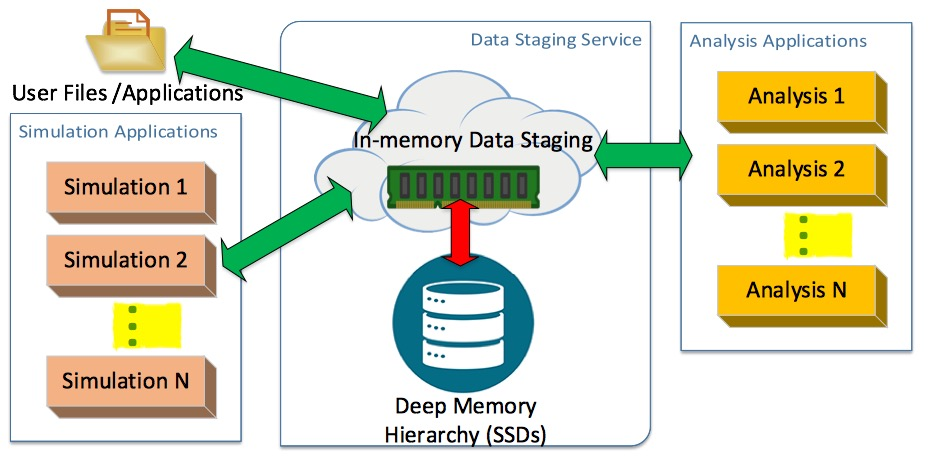
\includegraphics[width=\textwidth]{images/stacker_fig_1.jpg}
        \caption{A typical data staging framework with in-memory data staging. Each of the data staging nodes/servers is equipped with SSDs.}
\end{figure}
\end{frame} 
%------------------------------------------------

%------------------------------------------------
\begin{frame}
\frametitle{Bottlenecks and Challenges}
\begin{block}{Capacity restrictions for DRAM}
The extreme-scale data can easily exceed DRAM's capacity. Large amount of data must be offloaded/load between memory and burst buffers.
\end{block}

\begin{block}{Latency and throughput gap}
Burst buffers have much longer access latencies and lower throughput compared to main memory. Thus intelligent data prefetching based on access patterns can hide this disk access and data transfer latency.
\end{block}
%\begin{itemize}
%        \item The extreme-scale data can easily exceed DRAM's capacity. Large amount of data must be offloaded/load between memory and burst buffers.\\
%        \item Burst buffers have much longer access latencies and lower throughput compared to main memory. Thus intelligent data prefetching based on access patterns can hide this disk access and data transfer latency. \\
%        \item A component of the workflow which access offloaded data in burst buffer would benefit from efficient \textbf{prefetching} approches.
%        \item Current prefetching approches and their flaws:
%                \begin{enumerate}
%                        \item Methods based on user-defined hints. They work well for simple applications but struggle in complex tasks due to the manual tuning. \\
%                        \item Methods based on spatial/temporal locality. They work well with contiguous or fixed strided access patterns in a single application, whereas not effective for variable strided access nor in multi-application workflow.
%                \end{enumerate}
%\end{itemize}
\end{frame}
%------------------------------------------------
\begin{frame}
\frametitle{Related Works For Data Prefetching}
\begin{block}{Methods based on user-defined hints}
    They work well for simple applications but struggle in complex tasks due to the manual tuning. \\
\end{block}
\begin{block}{Methods based on spatial/temporal locality} 
    They work well with contiguous or fixed strided access patterns in a single application, whereas not effective for variable strided access nor in multi-application workflow.
\end{block}
\begin{block}{Methods based on N\textit{th}-order Markov chain}
    These works mainly risides in kernel space and do prefetching at the granularity of pages.        
\end{block}
\end{frame}
%------------------------------------------------
\begin{frame}
\frametitle{Contributions of \textit{Stacker}}
    \begin{itemize}
        \item \textit{Stacker} implements N-gram model for abstracting access patterns and predicting requests automatically.
        \item Rather than modeling individual applications and their access patterns, \textit{stacker} models the data accesses among mutiple components of application workflows.
    \end{itemize}

%The goal of this paper is to explore machine learning based approaches to capture the data access patterns between components of staging-based in-situ application workflows, and to use these learned access patterns to move data between the storage layers of the staging service in an autonomous manner.

\end{frame}
%------------------------------------------------
\section{Introduction to Stacker}
%\subsection{Main Architecture}
\begin{frame}
%\subsection{Overview}
\frametitle{Main Architecture}
\begin{figure}
        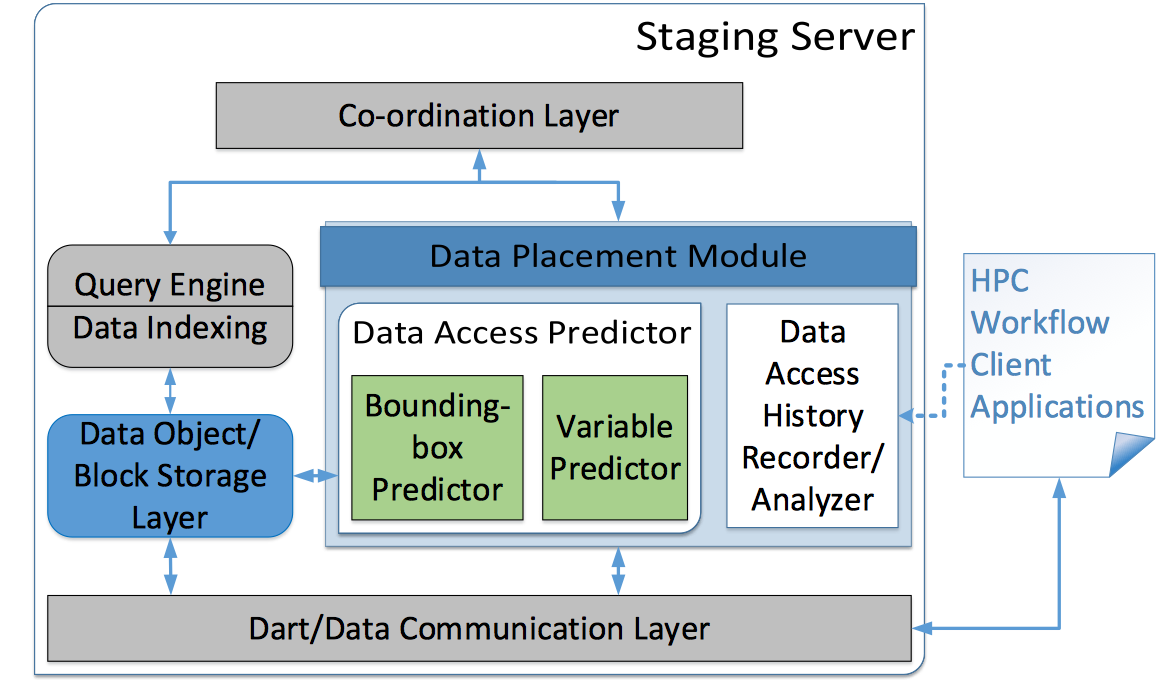
\includegraphics[width=\linewidth]{images/stacker_fig_2.png}
        \caption{Architecture of multi-tiered staging framework of Stacker}
\end{figure}
\end{frame}
%------------------------------------------------
\begin{frame}
\frametitle{\textit{Dataspaces}}
%\begin{block}{\textit{Dataspaces}}
%\textit{Data-Spaces} is the fundamental framework of data-staging services, which offers a virtual shared-space abstraction between DRAM and on-node SSDs.
%consists of query engine layer, data indexing layer and data storage layer.
%Data-Spaces is a flexible interaction and coordination substrate for end-to-end scientific workflows.
%\end{block}
\begin{figure}
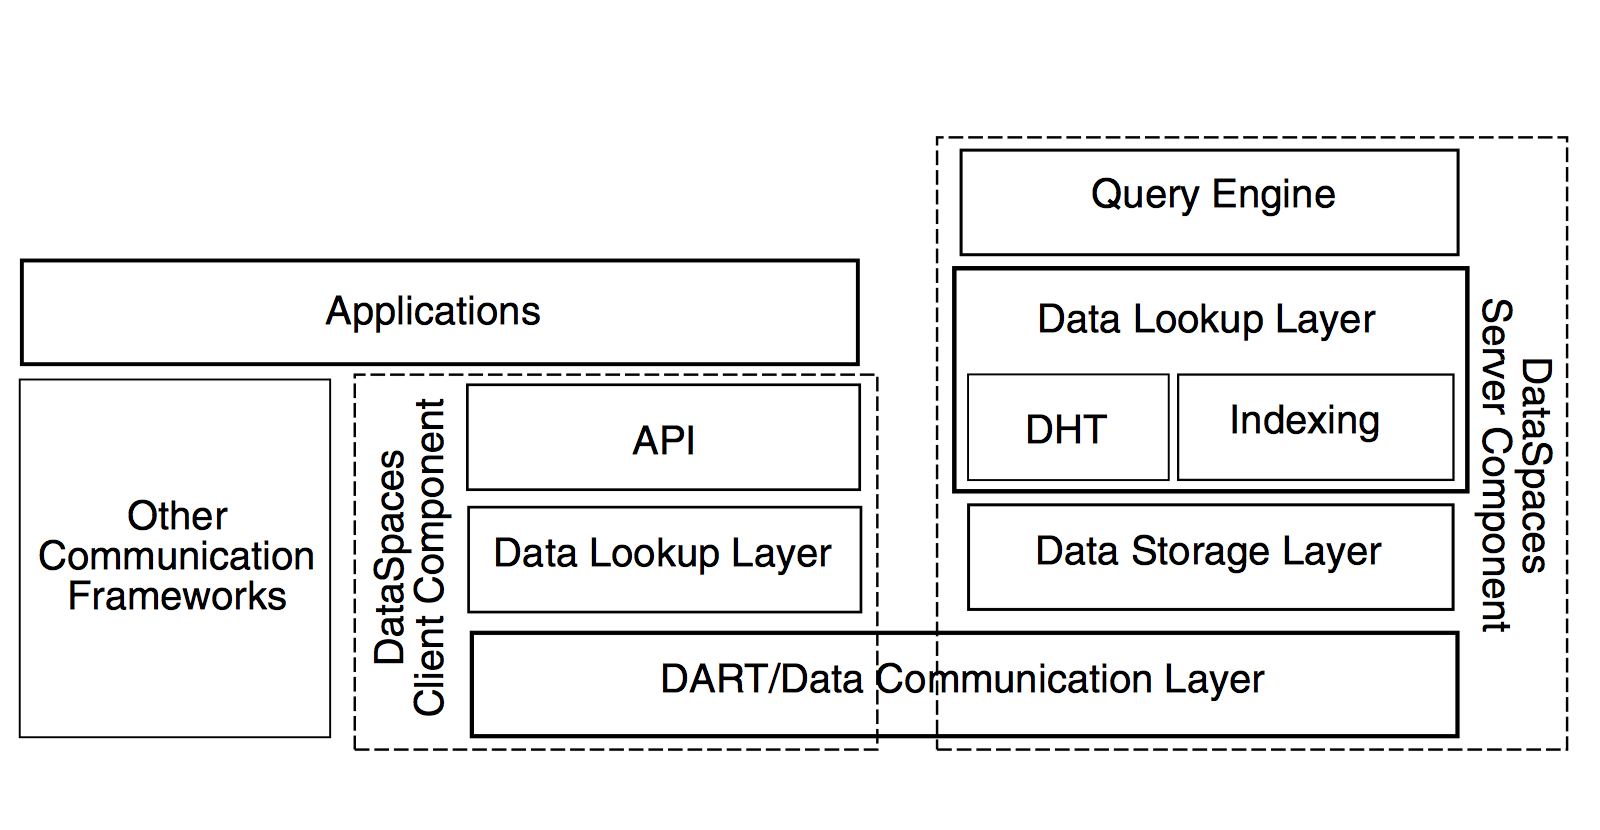
\includegraphics[width=\textwidth]{images/dataspaces.png}
\caption{\textit{Data-Spaces} is the fundamental framework of data-staging services, which offers a virtual shared-space abstraction between DRAM and on-node SSDs.}
\end{figure}
\end{frame}

%------------------------------------------------
\begin{frame}
\frametitle{Shared-space between DRAM and SSDs}
%            \begin{block}{Data Object/Block Storage Layer}
Within \textit{Data-Spaces}, a name conversion utility between in-meomory objects and in-storage files is implemented. By this means, data loading requests are analyzed and predicted in object/variable level rather than files. Metadata for files in data-staging servers are formed as below:
%            \end{block}
            \begin{tabular}{|c|c|}
                    \hline
                    \textbf{Metadata} & \textbf{Description} \\
                    \hline
                    DSG\_ID & ID of the server storing the object.\\
                    \hline
                    var\_name & name of the variable in workflow.\\
                    \hline
                    lb & Starting offset of the object in the global bounding box.\\
                    \hline
                    ub & Ending offset of the object.\\
                    \hline
                    ver & Version number of the object.\\
                    \hline
            \end{tabular}
%\par A bounding box is a geometric descriptor specifying the range of data along each dimension of the application domain. All of this information is concatenated into a string to create an unique file-name for each object. This object is then written as a file to the SSD using POSIX write APIs. When an object stored in SSD is requested, the file-name is functionally computed and appropriate data from that specific file is sent to the requesting client. 
\end{frame}
%------------------------------------------------
%\subsection{Data Placement Module}
\begin{frame}
%\subsubsection{Data Placement Module}
\frametitle{Data Placement Module}

%    \begin{block}{Data Placement Module}
%            This module records data access history(metadata) and implements efficient prefetching alogorithm to enhance the reading performance.
In this module, access history is stored in a hash-table for succeeding prediction. As an example, consider the case in which several applications are requesting data from variables: \textit{$\alpha \rightarrow \beta \rightarrow \gamma \rightarrow \delta$}, successively. 
\end{frame}

%------------------------------------------------
\begin{frame}
\frametitle{Step 1: Data Access History Recording/Analyzing}
Supppose we implement 4-gram model at most in this example. According to the requests $\alpha \rightarrow \beta \rightarrow \gamma \rightarrow \delta$, the 4-gram, 3-gram and 2-gram gram-frequency pairs in the hash-table are updated as below:
    \begin{center}
    \begin{table}
    \begin{tabular}{|c|c|}
            \textbf{Grams} & \textbf{Occurrence frequency} \\
            $\alpha, \beta, \gamma, \delta$ & +1 \\
            $\alpha, \beta, \gamma$ & +1 \\
            $\beta, \gamma, \delta$ & +1 \\
            $\alpha, \beta$ & +1 \\
            $\beta, \gamma$ & +1 \\
            $\gamma, \delta$ & +1 \\
            ... & ... \\
    \end{tabular}
    \caption{An hash-table for variable access history.}
    \end{table}
    \end{center}
%    \end{block}
          
\end{frame}

%------------------------------------------------
\begin{frame}
\frametitle{Step 2: Predicting}
            This algorithm is a \textit{hierarchical prediction} that would search for the previous grams as long as possible in the hash-table.
    \begin{center}
            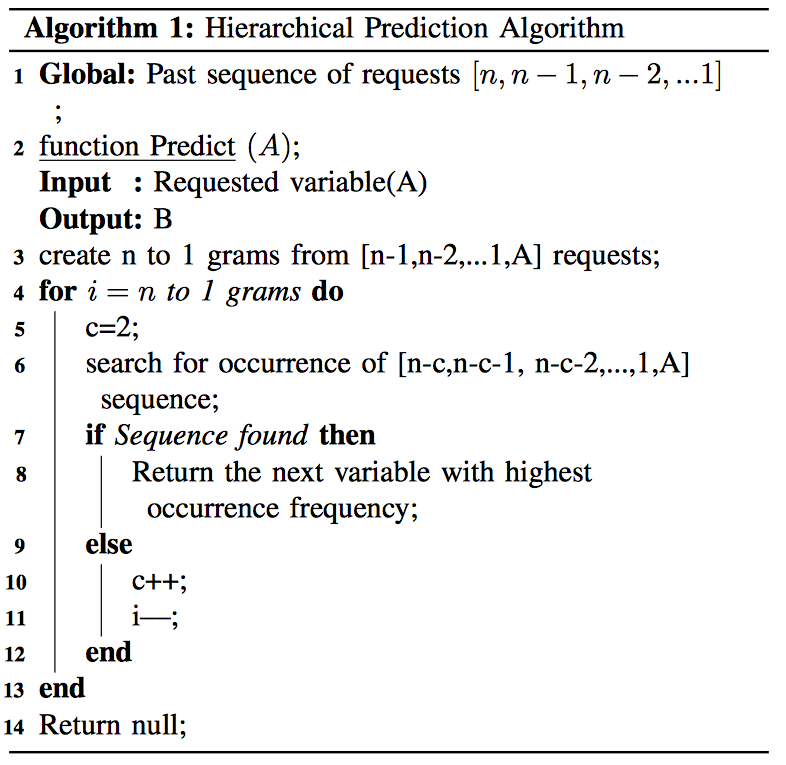
\includegraphics[width=.5\textwidth]{images/stacker_fig_3.png}
    \end{center}
%\end{column}
%\end{columns}
\end{frame}

%------------------------------------------------
\begin{frame}
%\begin{columns}
%\begin{column}{.5\textwidth}
\frametitle{Step 3: Prefetching and Evicting}
            A FIFO queue is maintained for the prefetch partition. The staging server runs two extra thread, one for prefetching predicted data from Step 2, and another for evicting the oldest data in cache.
\end{frame}

\section{Evaluation}
\begin{frame}
\frametitle{Evaluation}
To evaluate Stacker, both synthetic experiments and real scientific workflow were tested.
\begin{block}{Environment for Synthetic Experiment}
        The Caliburn Supercomputer at the Rutgers Discovery Informatics Institude, which consists of 560 nodes, each containing Dual Intel Xeon E5-2695v4, 18-Core processors with 256 GB of RAM and a 400GB Intel NVMe drive per node.
\end{block}
\begin{block}{Environment for Real Scientific Workflow}
Titan Cray XK7 system. It has 18,688 compute nodes and each node is equipped with 16-core AMD 6200 series Opteron processor and 32 GB memory. \\

They used the combustion DNS-LES simulation/analysis from the S3D comustion and analysis workflow.
\end{block}
\end{frame}

%------------------------------------------------
\begin{frame}
\frametitle{Synthetic Experiments}
\begin{center}
        \includegraphics*[width=\textwidth]{images/stacker_fig_4.png}
\end{center}
\end{frame}
%------------------------------------------------
\begin{frame}
\frametitle{Real Scientific Workflows}
\begin{center}
        \includegraphics*[width=\textwidth]{images/stacker_fig_5.png}
\end{center}
\end{frame}
%------------------------------------------------


%------------------------------------------------

%------------------------------------------------

%\begin{frame}[fragile] % Need to use the fragile option when verbatim is used in the slide
%\frametitle{Citation}
%An example of the \verb|\cite| command to cite within the presentation:\\~

%This statement requires citation \cite{p1}.
%\end{frame}

%------------------------------------------------

%\begin{frame}
%\frametitle{References}
%\footnotesize{
%\begin{thebibliography}{99} % Beamer does not support BibTeX so references must be inserted manually as below
%\bibitem[Smith, 2012]{p1} John Smith (2012)
%\newblock Title of the publication
%\newblock \emph{Journal Name} 12(3), 45 -- 678.
%\end{thebibliography}
%}
%\end{frame}

%------------------------------------------------

%\begin{frame}
%\Huge{\centerline{The End}}
%\end{frame}

%----------------------------------------------------------------------------------------

\end{document} 
